\documentclass[a4wide, 11pt]{article}
\usepackage{a4, fullpage}
\usepackage[pdftex]{graphicx}  
\usepackage[export]{adjustbox}
\usepackage{wrapfig}
\usepackage{lipsum}
\setlength{\parskip}{0.3cm}
\setlength{\parindent}{0cm}

% This is the preamble section where you can include extra packages etc.

\begin{document}

\title{Project Technology Report}

\author{Cardspark - Group 26}

\date{\today}         % inserts today's date

\maketitle            % generates the title from the data above

\section{Client-side}
\begin{itemize}
\item \textbf{Ruby on Rails}\\
We choose Rails as it allowed fast prototyping of our web application and followed the MVC architecture so it was easy to separate the view from the models and controllers.
\end{itemize}

\section{Server-side}
\begin{itemize}
\item \textbf{Swift}\\ 
\end{itemize}

\section{Version Control, Continuous Integration and Deployment}
\begin{itemize}
    \parbox[t]{\dimexpr\textwidth-\leftmargin}{%
      \vspace{-2.5mm}
      \begin{wrapfigure}[16]{r}{0.5\textwidth}
        \centering
        \vspace{-\baselineskip}
		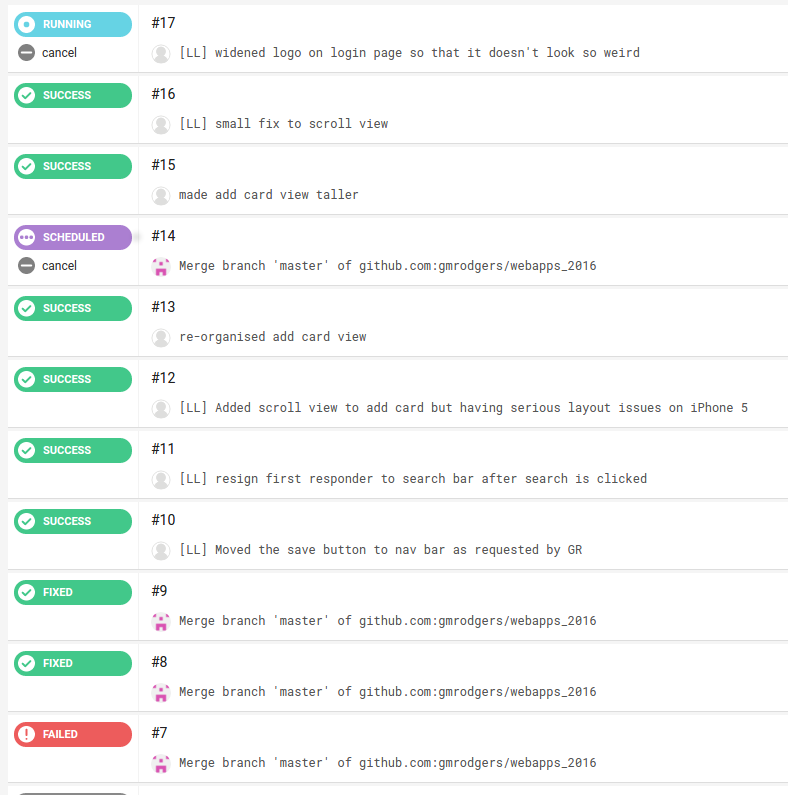
\includegraphics[scale=0.25]{builds.png}
        \caption{CircleCI builds}
      \end{wrapfigure}
\item \textbf{Github}\\
Used as our git repository hosting service as it provides free private repositories and we had used it before.
\item \textbf{CircleCI} (linked to github repo)\\
Used for continuous integration as it was easy to set up and works with Ruby on Rails.
\item \textbf{Code Climate} (linked to github repo)\\
Used by our group to monitor our overall code quality.  Allows us to see adjustments needed after every commit.
\item \textbf{Heroku} (linked to github repo)\\
We push to a remote Heroku repository which then deploys our backend onto its 
cloud platform.
    }
  \end{itemize}


\end{document}